\chapter{Testing}\label{chapter:testing}
Come anticipato nel paragrafo \ref{sec:postman}, il software utilizzato per la fase di testing del progetto è Postman.\\
L'utilizzo di questo software non è stato strettamente necessario, dato che si può ottenere lo stesso risultato effettuando da terminale un comando \texttt{curl} all'indirizzo di Kong Gateway, specificando tutti i parametri e i campi della richiesta \texttt{HTTP}, ottenendo comunque i risultati (in formato diverso).\\
L'utilizzo di Postman è stato preferito per motivi di comodità nella fase di testing, soprattutto perché offre la possibilità di memorizzare le richieste inviate (con tutti i relativi campi e parametri) e i risultati.\\
Il software risulta molto intuitivo, basta selezionare il metodo di richiesta che si vuole utilizzare (in questo caso \texttt{HTTP GET}), inserire l'URL e, se necessario, configurare i campi della richiesta, ovvero in questo caso, aggiungere al body della richiesta il token JWT.\\

Di seguito alcune immagini che dimostrano il funzionamento del progetto:\\
\begin{figure}[h]
	\centering
	\resizebox{0.6\textwidth}{!}{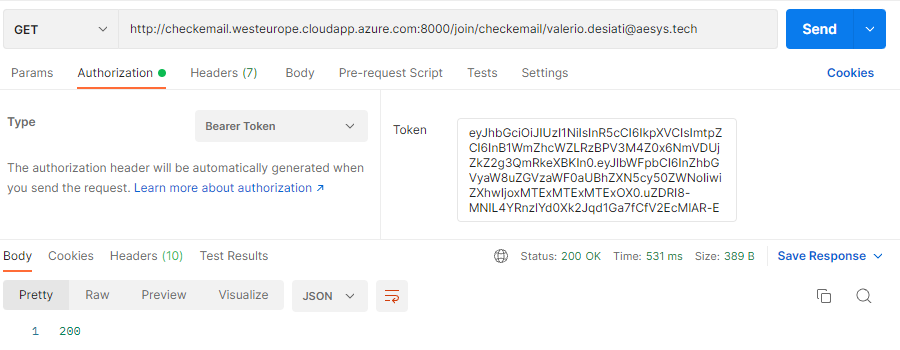
\includegraphics{img/postmanauthorized-cut.png}}
	\caption{Test - Autorizzazione concessa}
	\label{fig:one}
\end{figure}

\begin{figure}[h]
	\centering
	\resizebox{0.6\textwidth}{!}{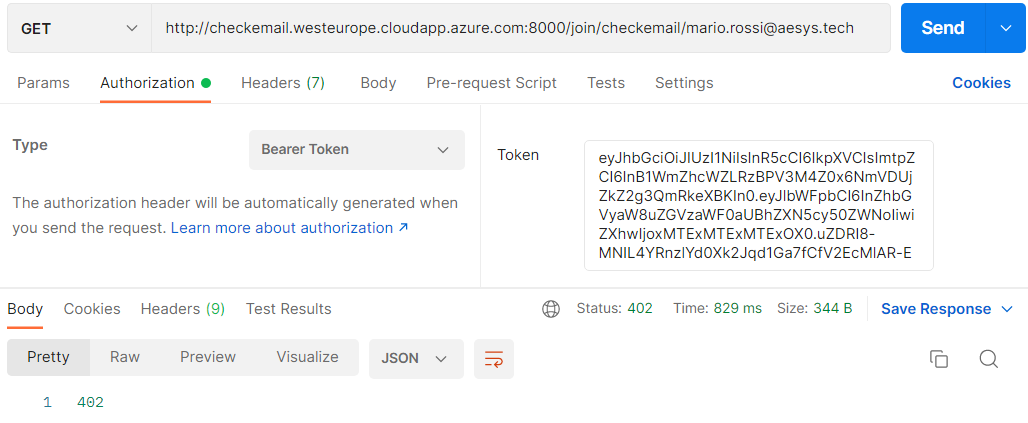
\includegraphics{img/postmanpaymentrequired-cut.png}}
	\caption{Test - Autorizzazione non concessa, pagamento richiesto}
	\label{fig:one}
\end{figure}

\begin{figure}[h]
	\centering
	\resizebox{0.6\textwidth}{!}{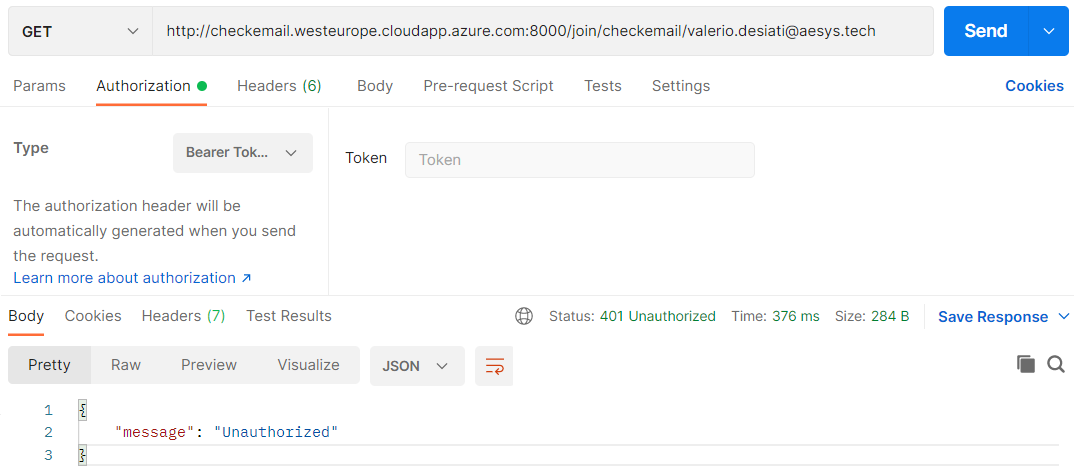
\includegraphics{img/postmanquerynotoken-cut.png}}
	\caption{Test - Autorizzazione non concessa, token non inserito}
	\label{fig:one}
\end{figure}



